
\chapter{FACT}

\section{Goal}
The aim of FACT is to be a solution for provide a system for use within a corporate setting that presents required information and company policies to the employees in small, easy to digest chunks. This is to solve the problem of informing employees of information and being able to check if employees have actually read the information as well as providing a platform for reference material or training. What Haunt found when they were going through the early stages of their company development process was that there was a lack of effective and efficient applications that are effective at informing employees of essential information in a corporate environment, such as health and safety and other company policies. They established that there was a market for a solution that addresses this need for a lightweight application that can be used as an on boarding education tool as well as continued education of company policies. The solution would also notify employees of changes to policies that are relevant to them and allow a manager to ensure that their staff were up to date with company policies. The product should also be scalable to contain enough information that is easily navigable that it could replace or be used in conjunction with other knowledge management systems such as company wikis.

\section{FACT - The Product}
FACT is a micro-learning management tool that offers the ability to manage information on company policies, procedure and other employee on boarding necessities. The final product will also keep track of what users have read, notify them of any changes to the information that needs to be read and allows an administrator to monitor user participation. This information will be organized into decks that would be similar to courses in a more fully fledged learning management system. These decks will be the topics that a user could have assigned to them as required for their role. Decks will be filled with chunks of information called cards and/or facts. These will have a word limit on them to promote smaller chunks of information so they users are more likely to read them.

\section{Features}
\subsection{Users and Organisations}
Organisations will be the account that a user will be registered under. Users under the same organisations will be able to access  the same resources such as decks, cards and tags. The users will be rather simple entities that can be linked to decks through tags and able to be assigned a role for their access rights. A user will need to keep track of the completed cards and when/what version of each card was completed.

\subsection{Decks, Cards and Tags}
Cards would only contain snippets of information that could be easily digestible and mark off as understood. Cards should present the information in a way that the user can easily view all the information and tick them off once they are understood. Cards could also have the ability to show media such as images or video. The editing and restrictions for the cards should promote the idea of this bite sized information. The aim of a card or fact is to convey information that is a self sufficient piece of information, further detailed information could be linked to provide a more thorough overview (See \ref{fig:pitchdecks}).

\begin{figure}[h]
\label{pitchdecks}
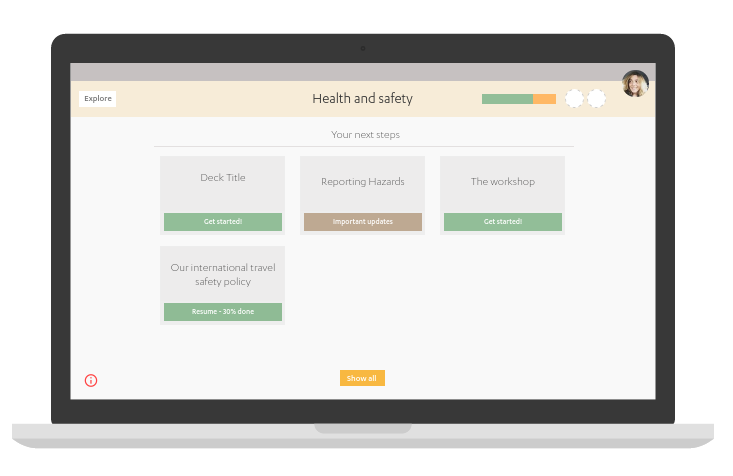
\includegraphics[width=\textwidth]{pitch-decks01}
\caption{The initial pitch concept for the display of decks}
\centering
\end{figure}

The way that the cards will be organized is with decks. Decks will be the underlying structure that represents topics and the cards within them would be related to those topics. For example a deck could be labeled ”Emergency plan” and the cards within could note the steps that need to be taken within different emergencies and other helpful tips and information.
Decks would also have the ability to be tagged. Tags would represent the over arching topics that the decks touches. Such as ”Heath and Safety” or ”PHP”.
\begin{figure}
\label{pitchcards}
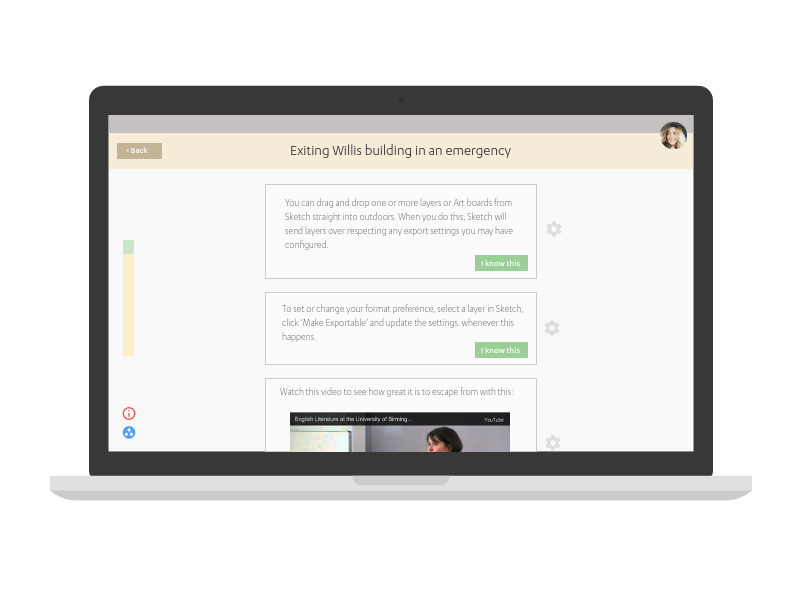
\includegraphics[width=\textwidth]{pitch-cards}
\caption{The initial pitch concept for the display of cards/facts}
\centering
\end{figure}
Tags associated with a decks allow for much more interaction with from the users and the decks. It would enable a user to ”subscribe” to certain tags, or a manager to decide what tagged decks are mandatory or recommended for an employee to complete and other similar actions.



